\section{Consuntivazione}

\subsection{Milestones:}
\begin{itemize}
    \item Release versione 0.0.4 dell'analisi dei requisiti (Completa al: 75\%)
\end{itemize}

\subsection{Attività svolte}

\begin{table}[ht]
    \begin{tabularx}{\textwidth}{X l l}
        
        \rowcolor{gray!30} \textbf{Attività} & \textbf{Stato} & \textbf{Ruolo}\\
        
        \hline
        creazione e manutenzione workflow amministrativi & completato & Amministratore\\
        confronto con propontente & completato & Analista\\
        contronto con committente & completato & Analista\\
        \end{tabularx}
    \caption{Lista delle attività svolte durante lo sprint}
\end{table}


\begin{table}[ht]
    \begin{tabularx}{\linewidth}{X|rrrrrrr}
    \rowcolor{gray!30}& Re & Amm & An & Pro & Prog & Ver & tot \\
    \hline
    Bonavigo Michele                        & 0 & 0 & 0 & 0 & 0 & 1,35  & 1,35 \\
    \rowcolor{gray!10}Casarotto Mattia      & 3,9 & 0 & 0 & 0 & 0 & 0  & 3,9 \\
    Massarenti Alessandro                   & 0 & 0 & 1,3 & 0 & 0 & 0,5  & 1,8 \\
    \rowcolor{gray!10}Peron Samuel          & 0 & 0 & 0 & 0 & 0 & 0 & 0 \\
    Pierobon Luca                           & 0 & 2,25 & 0 & 0 & 0 & 0 & 2,25 \\
    \rowcolor{gray!10}Romano Davide         & 0 & 0 & 0 & 0 & 0 & 0 & 0 \\
    Zarantonello Giorgio                    & 0 & 0 & 0 & 0 & 0 & 0 & 0 \\
    \hline                                  & 3,9 & 2,25 & 1,3 & 0 & 0 & 1,85 & 
    \end{tabularx}
    \caption{\label{ruoli-persone}Spartizione dei ruoli e ore svolte durante lo sprint}
\end{table}

\begin{center}
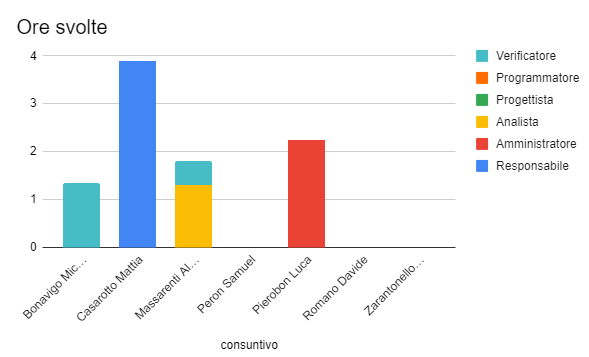
\includegraphics[width=12cm]{img/ore-svolte.png}
\end{center}

\begin{table}[ht]
    \begin{tabularx}{\linewidth}{X|l|l}
    \rowcolor{gray!30}& Ore & Costo \\
    \hline
    
    Responsabile & 3,9 & € 117,00 \\
    \rowcolor{gray!10}Amministratore & 2,25 & € 45,00 \\
    Analista & 1,3 & € 32,50 \\
    \rowcolor{gray!10}Progettista & 0 & € 0,00 \\
    Programmatore & 0 & € 0,00 \\
    \rowcolor{gray!10}Verificatore & 1,85 &€ 27,75 \\
    totale & 9,3 & € 222,25 \\
    \end{tabularx}
    \caption{\label{costi-ruolo}Spartizione dei ruoli e ore svolte durante lo sprint}
\end{table}


Avendo quindi consumato €222,25\footnote{Si veda tabella \ref{costi-ruolo}} del budget durante questo sprint, rimangono ancora a disposizione € 12780,50 per gli sprint seguenti.

\subsection{Difficoltà e problemi di sprint}

Alcune questioni sono risultate durante questo sprint:

\begin{itemize}
    \item Conciliare impegni personali per incontri.
\end{itemize}

Queste verranno discusse in sede di preparazione del prossimo sprint.
